\chapter{Forskningsmetoder}
\label{ch:method}
Dette kapittelet redegjør for forskningsmetodene til prosjektet. Forskningsstrategiene og datagenereringsmetodene
tar utgangspunkt i \citet{oates}. Se figur \ref{fig:oates_model} for en oversikt over forskningsrammeverket.

\begin{figure}
\centering
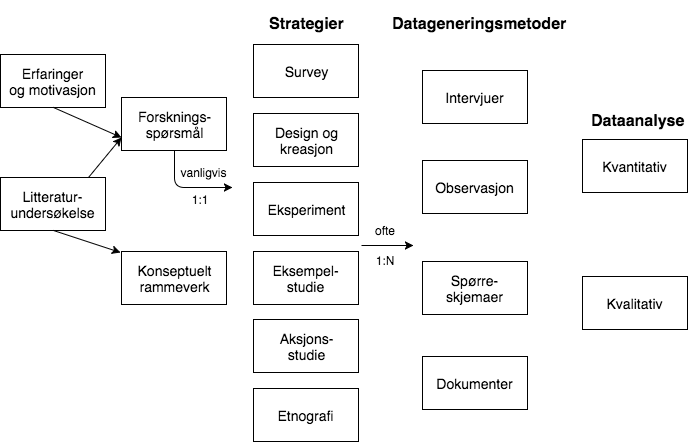
\includegraphics[width=0.90\textwidth]{fig/oates/oates_research_norwegian}
\caption{Modell av forskningsprosessen fra \citet{oates}.}
\label{fig:oates_model}
\end{figure}

\section{Forskningsstrategier}

\subsection{Design og kreasjon}
\textquote[\cite{oates}]{Forskningsmetoden design og kreasjon fokuserer på utvikling av nye IT-produkter, også kalt \textit{artefakter}.
Typer IT-artifakter inkluderer (March \& Smith, 1995): begreper, modeller, metoder og implementasjoner}{.}
Hovedpoenget er å lære gjennom å lage, og \citet{oates} identifiserer fem steg for denne prosessen:

\begin{description}
  \item[Bevisstgjøring] Hva er problemet?
  \item[Forslag] Hvordan kan problemet løses?
  \item[Utvikling] Problemløsingsfasen
  \item[Evaluering] Hvordan gikk dette?
  \item[Konklusjon] Hva kan vi trekke ut av dette?
\end{description}

\subsection{Case-studie}
Yin (2003) definerer i følge \citet{oates} case-studie som \textquote{en empirisk undersøkelse
som utforsker et samtidsfenomen i kontekst til virkeligheten, spesielt når grensene mellom fenomenet
og konteksten ikke er helt klart}{.}
\textquote[\cite{oates}]{En case-studie fokuserer på én instans av det som skal undersøkes: en organisasjon, en avdeling, et informasjonssystem,
    et diskusjonsforum (...). Denne ene instansen, eller tilfellet, studeres i detalj med forskjellige datagenereringsmetoder som
    intervju, observasjon, dokumenter (...)}{.}

Det som kjennetegner en case-studie er at det mer fokus på dybde snarere enn bredde,
at casen undersøkes i en naturlig ramme på en helhetlig måte, med flere kilder og metoder \citep[s. 142]{oates}. En undersøkende case-studie er nyttig for å kunne forstå
forskningsområdet bedre og definere gode forskningsspørsmål,
spesielt dersom det eksisterer lite forskning allerede, mens en beskrivende studie vil rette seg mer
mot å belyse én sak fra flere sider i en helhetlig historie. Den siste typen
case-studie er forklarende, og ønsker å finne ut hvorfor noe spesielt skjedde og hva
som forårsaket det \citep[s. 143]{oates}.
    
\subsection{Prototyping}

\subsection{Brukersentrert utvikling}
Brukersentrert utvikling er en prosess der brukeren er involvert i hvert steg.
Stegene er å forstå brukskonteksten, etablere krav, implementere artefakt og evaluere artefakt. Dette er en syklus som kan gjentas flere ganger.
\citet{dis20099241} standardiserer brukersentrert utvikling. Se figur \ref{fig:iso9241-210}
for de ulike stegene i prosessen.
Brukersentrert utvikling passer godt i de fem stegene som inngår i «design og kreasjon»-forskningsmetoden.

\begin{figure}
\centering
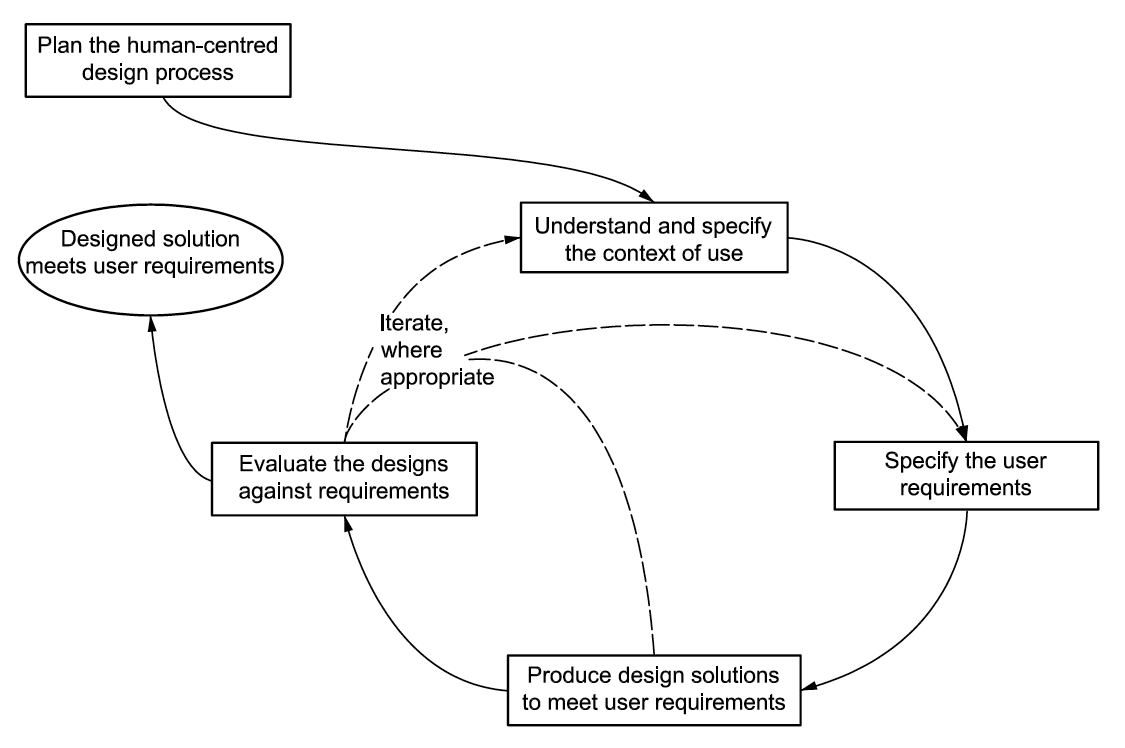
\includegraphics[width=0.85\textwidth]{fig/iso9241-210}
\caption{Gjensidige avhengigheter innenfor menneskeorientert designaktiviteter \citep{dis20099241}.}
\label{fig:iso9241-210}
\end{figure}

\section{Datagenereringsmetoder}

\subsection{Semistrukturert intervju}
Det finnes flere forskjellige typer intervju. Semistrukurert intervju er en datagenereringsmetode
der temaer og spørsmål er forberedt på forhånd, men rekkefølgen spørsmålene stilles i kan endre seg
og nye temaer og spørsmål kan komme opp basert på samtalen man har med intervjuobjektet. Det er et
kompromiss mellom et strukturert intervju og et helt ustrukturert intervju \citep[s. 188]{oates}.

Det er en mye brukt metode i case-studier for å få detaljert informasjon ut av intervjuobjektet.
I tillegg kan metoden brukes til å få tilbakemeldinger fra brukere på en kravspesifikasjon og en
endelige prototype \citep[s. 187]{oates}.

\subsection{Dokumenter}
